% id: 199-e2
% book: 개념원리 대수 · 21 사인법칙
% section: 필수·발전 예제
% figure: crop:fig-199-e2.png
% answer: $2$
% answer_source: 본문 풀이
% variant_level: 0 (원본 전사)
% 이 파일은 build.mjs 가 items.json 에서 만든다. 고칠 때는 items.json 을 고친다.
\smash{\raisebox{4.5mm}{\dmkichul{개념원리 대수 199쪽 예제 2 · 필수}}}
\noindent\begin{minipage}[t]{0.58\linewidth}\vspace{0pt}\raggedright 오른쪽 그림과 같이 $\seg{BC}=2\sqrt{2}$, $B=60^\circ$, $C=75^\circ$인 삼각형~$\pt{ABC}$의 외접원의 반지름의 길이 $R$를 구하시오.\end{minipage}\hfill\begin{minipage}[t]{0.4\linewidth}\vspace{0pt}\centering \setlength{\dmfigw}{64.1pt}\ifdim\dmfigw>\linewidth\setlength{\dmfigw}{\linewidth}\fi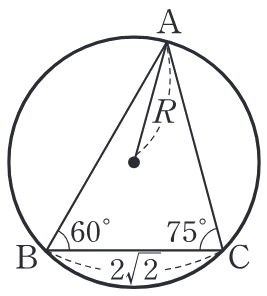
\includegraphics[width=\dmfigw]{figures/fig-199-e2.png}\end{minipage}\par
